\chapter{کلیّات}

\section{مقدمه}

شطرنج یکی از محیط‌های مناسب برای مطالعه و ارزیابی سامانه‌های هوش مصنوعی به شمار می‌رود؛ زیرا هر موقعیت شطرنجی دارای ساختاری مشخص و قابل تحلیل است و کیفیت یک حرکت را می‌توان با استفاده از قواعد بازی و موتورهای تخصصی شطرنج بررسی کرد. در سال‌های اخیر، عالوه بر استفاده از موتورهای شطرنج برای تعیین بهترین حرکت، توجه به تولید توضیحات قابل فهم برای بازیکن نیز افزایش یافته است. در این رویکرد، هدف تنها مشخص کردن درست یا نادرست بودن یک حرکت نیست، بلکه لازم است دلیل مناسب بودن یا نبودن آن نیز به زبانی قابل درک برای کاربر بیان شود.

با ظهور مدل‌های زبانی، امکان استفاده از این مدل‌ها برای تولید توضیحات متنی درباره موقعیت‌های شطرنجی فراهم شده است. این مدل‌ها از نظر توانایی تولید متن و دنبال کردن دستورها عملکرد قابل توجهی دارند؛ بااین‌حال، تولید یک متن روان لزوماً به معنای صحیح بودن تحلیل شطرنجی آن نیست. یک مدل زبانی ممکن است توضیحی از نظر زبانی مناسب تولید کند، اما در آن ویژگی‌هایی از صفحه، تهدیدهای تاکتیکی یا پیامدهای واقعی یک حرکت را نادرست بیان نماید. بنابراین، یکی از چالش‌های اصلی در این حوزه، ارزیابی هم‌زمان کیفیت زبانی و صحت محتوای شطرنجی توضیحات تولید شده است.

از سوی دیگر، مقایسه مدل‌های زبانی مختلف برای یک مسئله یکسان، بدون وجود مجموعه آزمون و معیار ارزیابی مشترک، می‌تواند نتایج نامنظم و دشواری در مقایسه ایجاد کند. به همین دلیل، وجود یک مجموعه‌داده ارزیابی کنترل‌شده که شامل موقعیت‌های مختلف شطرنجی، سطوح متفاوت بازیکنان و توضیحات مرجع باشد، اهمیت زیادی دارد.

در این پروژه، یک سامانه نرم‌افزاری برای تولید و ارزیابی توضیحات شطرنجی طراحی شده است که در آن تحلیل موتور شطرنج با مدل‌های زبانی ترکیب می‌شود. همچنین یک مجموعه آزمون شامل  ۶۰نمونه از موقعیت‌ها و حرکات شطرنجی تهیه و برای مقایسه چندین مدل زبانی مورد استفاده قرار گرفته است. در نهایت، خروجی مدل‌ها با استفاده از یک مدل زبانی مستقل و بر اساس معیارهای مشخص ارزیابی شده است. هدف اصلی این فرایند، ایجاد روشی یکسان برای بررسی توانایی مدل‌های زبانی در تولید توضیحات صحیح و مفید درباره حرکات شطرنج است.

\section{بیان مسئله}

یکی از کاربردهای مهم سامانه‌های هوشمند شطرنج، کمک به بازیکن برای درک دلیل مناسب یا نامناسب بودن یک حرکت است. موتورهای شطرنجی مانند  \lr{Stockfish}می‌توانند موقعیت صفحه را با دقت بالا تحلیل کرده و حرکت‌های مناسب، تغییر ارزیابی موقعیت و خطوط اصلی بازی را مشخص کنند؛ اما خروجی چنین موتورهایی معمولاً به شکل عدد، حرکت پیشنهادی یا خط بازی ارائه می‌شود و لزوماً توضیح آموزشی و قابل فهمی برای یک بازیکن انسانی فراهم نمی‌کند.

این مسئله به‌خصوص برای بازیکنان مبتدی و متوسط اهمیت بیشتری دارد. بازیکن ممکن است بداند که یک حرکت باعث کاهش ارزیابی موقعیت شده است، اما برای یادگیری از اشتباه خود نیاز دارد بداند چرا این حرکت مشکل داشته است؛ برای مثال، آیا مهره‌ای بدون دفاع باقی مانده، ساختار پیاده‌ای ضعیف شده، امنیت شاه کاهش یافته یا یک فرصت تاکتیکی از دست رفته است.

بنابراین، تبدیل اطلاعات دقیق موتور شطرنج به توضیحی قابل فهم برای انسان، یک مسئله مهم در مسیر استفاده آموزشی از سامانه‌های هوشمند شطرنجی است.

مدل‌های زبانی می‌توانند برای حل این بخش از مسئله مورد استفاده قرار گیرند؛ زیرا توانایی تولید متن طبیعی و تبدیل اطلاعات ساختار یافته به توضیحات قابل فهم را دارند. بااین‌حال، استفاده مستقیم از مدل‌های زبانی با یک مشکل اساسی همراه است: توانایی تولید متن روان الزاماً ً نشان‌دهنده توانایی تحلیل صحیح موقعیت شطرنجی نیست. مدل ممکن است اطلاعاتی را تولید کند که از نظر زبانی منطقی به نظر برسد، اما با وضعیت واقعی صفحه یا تحلیل موتور شطرنج سازگار نباشد. این مسئله در ارزیابی مدل‌ها اهمیت زیادی دارد، زیرا مقایسه صرفاً بر اساس روان بودن متن نمی‌تواند کیفیت واقعی توضیحات شطرنجی را مشخص کند.

از طرف دیگر، مدل‌های زبانی موجود از نظر اندازه، معماری، قابلیت استدالل و هزینه اجرای محلی تفاوت قابل توجهی دارند. در نتیجه، انتخاب یک مدل مناسب برای تولید توضیحات شطرنجی نیازمند آزمایش مدل‌های مختلف بر روی ورودی‌ها و نمونه‌های یکسان است. در صورتی که مجموعه آزمون مناسبی وجود نداشته باشد، مقایسه مدل‌ها به‌شکل قابل اعتماد دشوار خواهد بود.

در این پروژه، مسئله اصلی به‌صورت زیر تعریف می‌شود:

چگونه می‌توان یک سامانه و فرایند ارزیابی طراحی کرد که در آن مدل‌های زبانی مختلف، با استفاده از اطلاعات واقعی و قابل بررسی شطرنجی، توضیحاتی درباره حرکات تولید کنند و این توضیحات بر اساس معیارهای یکسان از نظر صحت، مفید بودن و کیفیت زبانی با یکدیگر مقایسه شوند؟

برای پاسخ به این مسئله، لازم است چند چالش به‌صورت هم‌زمان مورد توجه قرار گیرد. نخست، نمونه‌های آزمون باید شامل موقعیت‌ها و حرکات متنوع باشند و سطوح مختلف بازیکنان را پوشش دهند. دوم، برای هر نمونه باید اطلاعات کافی از وضعیت قبل و بعد از حرکت و تحلیل شطرنجی آن وجود داشته باشد. سوم، برای مقایسه خروجی مدل‌ها به یک توضیح مرجع نیاز است که بتوان خروجی تولید شده را با آن مقایسه کرد. در نهایت، ارزیابی باید تا حد امکان مستقل از خود مدل تولیدکننده انجام شود.

بر این اساس، در این پروژه مجموعه‌ای متوازن شامل  ۶۰نمونه از بازی‌های واقعی شطرنج ایجاد شده که  ۲۰نمونه مربوط به هر یک از سطوح مبتدی، متوسط و پیشرفته است. برای هر نمونه، اطلاعات موقعیت قبل و بعد از حرکت، خود حرکت و اطلاعات تحلیلی مرتبط در نظر گرفته شده و توضیح مرجع آموزشی نیز تدوین شده است. سپس مدل‌های زبانی مختلف با استفاده از یک فرایند یکسان آزمایش شده و خروجی آن‌ها توسط یک مدل زبانی مستقل ارزیابی شده است.

وجه تمایز اصلی این پروژه در تمرکز هم‌زمان بر تولید توضیح، ایجاد مجموعه‌داده ارزیابی، مقایسه مدل‌های مختلف و ارزیابی مستقل خروجی‌ها است. همچنین در معماری پیشنهادی، اطلاعات حاصل از موتور شطرنج پیش از ارسال به مدل زبانی پردازش و به‌صورت ساختاریافته در اختیار آن قرار می‌گیرد تا مدل به جای تکیه صرف بر دانش زبانی خود، از شواهد قابل بررسی مربوط به موقعیت شطرنجی نیز استفاده کند.

\section{کلیات روش پیشنهادی}

هدف این پروژه، طراحی و پیاده‌سازی یک پایپالین نرم‌افزاری برای تحلیل موقعیت‌های شطرنج، تولید توضیحات زبانی و ارزیابی نظام‌مند مدل‌های زبانی است. روش پیشنهادی از دو پایپالین مرتبط تشکیل می‌شود. پایپالین نخست برای ساخت مجموعه آزمون مرجع و ارزیابی مدل‌های مختلف به کار می‌رود. پایپالین دوم نیز فرایند استفاده واقعی از سامانه را از زمان دریافت موقعیت یا حرکت از کاربر تا نمایش توضیح نهایی مدیریت می‌کند.

\subsubsection*{. ۱پایپالین ارزیابی مدل‌ها}

پایپالین ارزیابی مدل‌ها خود از دو فاز تشکیل شده است: فاز نخست به ساخت مجموعه آزمون مرجع اختصاص دارد و در فاز دوم، مدل‌های زبانی با استفاده از این مجموعه آزمایش و مقایسه می‌شوند.

\subsubsection*{فاز اول: ساخت مجموعه آزمون مرجع}

در نخستین مرحله، بازی‌های واقعی شطرنج بررسی شد و از میان آن‌ها  ۶۰حرکت یا موقعیت برای تشکیل مجموعه آزمون انتخاب شد. نمونه‌ها به‌گونه‌ای انتخاب و دسته‌بندی شد که بازیکنان با سطوح مهارتی مختلف و انواع متنوعی از حرکات، اشتباهات و موقعیت‌های تاکتیکی و استراتژیک در مجموعه حضور داشته باشند. برای هر نمونه، اطلاعاتی مانند وضعیت صفحه پیش از حرکت، حرکت انجام‌شده، وضعیت صفحه پس از حرکت و سایر داده‌های لازم ذخیره شد.

در مرحله بعد، وضعیت صفحه پیش و پس از هر حرکت با استفاده از موتور شطرنج  \lr{Stockfish}تحلیل شد. این تحلیل شامل امتیاز موقعیت، بهترین حرکت پیشنهادی، خطوط اصلی بازی، تغییر امتیاز پس از حرکت و میزان فاصله حرکت بازیکن با انتخاب پیشنهادی موتور است.

پس از دریافت تحلیل، \lr{Stockfish}اطلاعات مربوط به دو وضعیت قبل و بعد از حرکت با یکدیگر مقایسه شدند. در این مرحله، ویژگی‌های مهم شطرنجی مانند تغییر ارزیابی موقعیت، جابه‌جایی یا از دست رفتن مهره‌ها، ساختار پیاده‌ای، امنیت شاه، کنترل خانه‌های مهم، تهدیدهای ایجاد شده و برخی الگوهای تاکتیکی و موقعیتی استخراج می‌شوند.

سپس هر یک از  ۶۰نمونه به‌صورت انسانی بررسی و برچسب‌گذاری می‌شود. برای هر موقعیت، یک پاسخ مرجع شامل توضیح مناسب درباره حرکت، پیامدهای آن و دلایل احتمالی خوب یا نامناسب بودن حرکت تهیه می‌شود. در پایان این فاز، مجموعه آزمون مرجع شامل داده‌های شطرنجی، نتایج تحلیل، \lr{Stockfish}ویژگی‌های استخراج‌شده و توضیح انسانی آماده خواهد بود.

\subsubsection*{فاز دوم: آزمون و مقایسه مدل‌ها}

پس از آماده‌شدن مجموعه آزمون مرجع، مدل زبانی مورد ارزیابی روی همان  ۶۰نمونه اجرا می‌شود. برای هر نمونه، اطلاعات حاصل از  \lr{Stockfish}و ماژول استخراج ویژگی در قالب یک ورودی ساختاریافته در اختیار مدل قرار

می‌گیرد. این ورودی می‌تواند شامل وضعیت صفحه، حرکت بازیکن، تغییر امتیاز، بهترین حرکت پیشنهادی موتور و ویژگی‌های تاکتیکی و موقعیتی استخراج‌شده باشد.

مدل مورد آزمایش با استفاده از این اطلاعات، توضیحی متنی درباره حرکت تولید می‌کند. خروجی‌های مدل در قالبی مشخص دریافت، ذخیره و یکسان‌سازی می‌شوند تا تفاوت‌های ظاهری یا ساختاری مانع ارزیابی منصفانه مدل‌ها نشوند. این فرایند برای تمام نمونه‌های مجموعه آزمون و برای هر مدل زبانی مورد بررسی تکرار می‌شود.

در مرحله ارزیابی، توضیح تولید شده توسط هر مدل با پاسخ انسانی مرجع همان نمونه مقایسه می‌شود. برای انجام این مقایسه، مدل مستقل  \lr{Gemma 4 12B}به‌عنوان داور به کار می‌رود. این مدل بر اساس معیارهای از پیش تعیین‌شده، میزان تطابق پاسخ مدل با پاسخ مرجع را بررسی می‌کند. معیارهای ارزیابی می‌توانند شامل صحت شطرنجی، ارتباط توضیح با حرکت، پوشش نکات اصلی، نبود ادعاهای نادرست، وضوح متن و میزان شباهت محتوایی به پاسخ مرجع باشند.

در پایان، خطاها و امتیازهای هر مدل محاسبه می‌شوند. نتایج به‌صورت تجمیعی و در سطح هر نمونه ذخیره می‌شوند تا مقایسه مدل‌ها، شناسایی نقاط ضعف آن‌ها و انتخاب مناسب‌ترین مدل برای استفاده در سامانه امکان‌پذیر باشد.

\subsubsection*{. ۲پایپالین استفاده واقعی}

پایپالین دوم مربوط به زمانی است که کاربر از سامانه استفاده می‌کند. در این حالت، کاربر یک حرکت یا موقعیت شطرنجی را وارد می‌کند. ورودی می‌تواند شامل وضعیت صفحه و حرکت انجام‌شده یا وضعیت صفحه پیش و پس از حرکت باشد.

این اطلاعات ابتدا برای تحلیل به  \lr{Stockfish}ارسال می‌شوند. موتور شطرنج وضعیت موجود، کیفیت حرکت، بهترین ادامه‌های ممکن و تغییر ارزیابی ناشی از حرکت را مشخص می‌کند. سپس خروجی موتور وارد ماژول پردازش شطرنج می‌شود.

ماژول پردازش، خروجی  \lr{Stockfish}و اطلاعات صفحه را بررسی می‌کند و با استفاده از قواعد اکتشافی، ویژگی‌های قابل توضیح را استخراج می‌کند. این قواعد می‌توانند برای تشخیص مواردی مانند از دست رفتن مهره، ایجاد تهدید، ضعف امنیت شاه، تغییر ساختار پیاده‌ای، کنترل خطوط باز یا شکل‌گیری یک الگوی تاکتیکی استفاده شوند.

داده‌های حاصل در قالب یک ورودی ساختاریافته به مدل زبانی منتخب ارسال می‌شوند. این مدل همان مدلی است که بر اساس نتایج پایپالین ارزیابی، عملکرد مناسب‌تری داشته است. مدل زبانی با تکیه بر اطلاعات ارائه‌شده، توضیحی قابل‌فهم درباره حرکت تولید می‌کند و متن نهایی از طریق رابط کاربری به کاربر نمایش داده می‌شود.

\subsubsection*{معماری نرم‌افزاری سامانه}

معماری کلی نرم‌افزار شامل موتور تحلیل شطرنج، ماژول استخراج ویژگی و قواعد اکتشافی، بخش ساخت ورودی، ماژول ارتباط با مدل‌های زبانی، پایگاه ذخیره نتایج \lr{Backend}، برای مدیریت پردازش‌ها و \lr{API}ها و  \lr{Frontend}برای تعامل کاربر با سامانه است.

تفکیک این بخش‌ها باعث می‌شود مدل زبانی، موتور شطرنج یا معیارهای ارزیابی بدون ایجاد تغییر اساسی در کل سامانه جایگزین یا اصلاح شوند. همچنین می‌توان مدل‌های مختلف را با ورودی‌ها، تنظیمات و معیارهای یکسان آزمایش کرد و نتایج آن‌ها را در شرایط قابل‌مقایسه به دست آورد.

روند کلی روش پیشنهادی در شکل~\ref{fig:intro-flow} نمایش داده شده است.
\begin{figure}[htbp]\centering
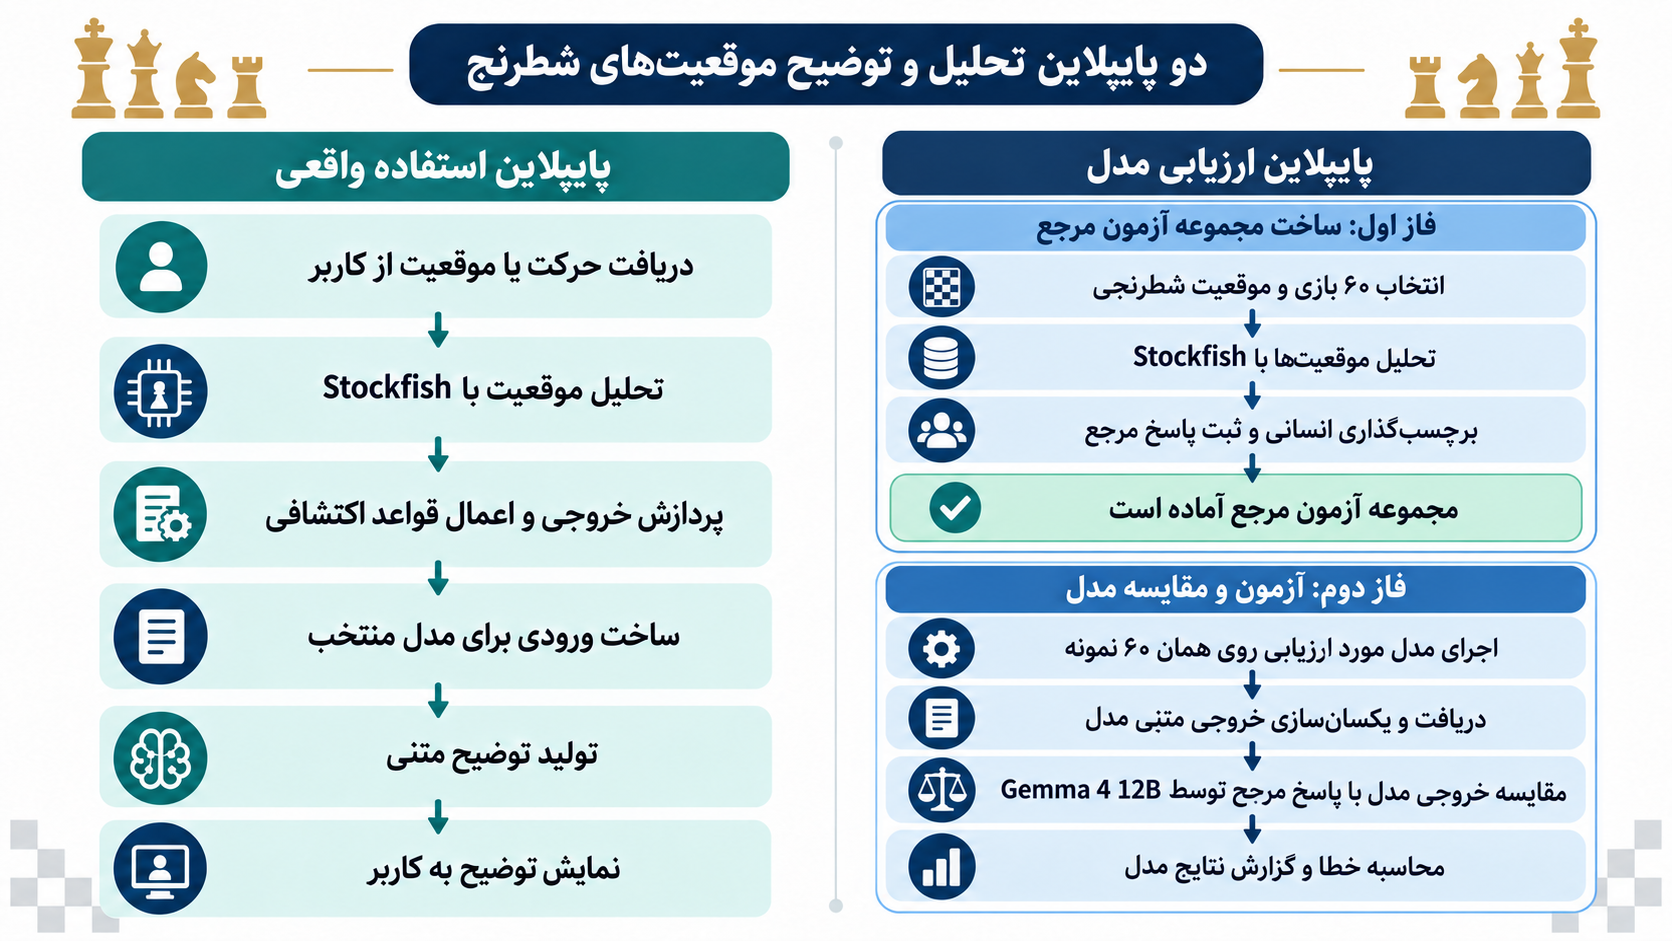
\includegraphics[width=\linewidth]{chapter3_assets/original_intro.png}
\caption{روند کلی ساخت، ارزیابی و استفاده از سامانه}\label{fig:intro-flow}
\end{figure}

بنابراین، خروجی نهایی پروژه صرفاً یک مدل تولیدکننده توضیحات شطرنجی نیست، بلکه یک سامانه نرم‌افزاری و چارچوب آزمایشی یکپارچه است. این سامانه از یک سو موقعیت‌های شطرنج را تحلیل کرده و توضیح قابل‌فهمی در اختیار کاربر قرار می‌دهد و از سوی دیگر، امکان آزمایش، ارزیابی و مقایسه مدل‌های زبانی مختلف را با استفاده از یک مجموعه آزمون مرجع فراهم می‌کند.

\section{ساختار پروژه}

این گزارش در سه فصل اصلی تنظیم شده است. در فصل اول، کلیات پروژه شامل مقدمه، بیان مسئله، هدف و روش پیشنهادی و همچنین ساختار گزارش ارائه می‌شود.

در فصل دوم، مفاهیم و فناوری‌های مرتبط با پروژه بررسی می‌شوند. در این فصل ابتدا مفاهیم پایه مرتبط با تحلیل شطرنج، موتورهای شطرنج، مدل‌های زبانی و تولید توضیحات متنی معرفی شده و سپس پژوهش‌ها و سامانه‌های مشابه مورد بررسی و مقایسه قرار می‌گیرند. هدف این فصل، مشخص کردن جایگاه پروژه حاضر در میان روش‌ها و سامانه‌های موجود است.

در فصل سوم، روش پیشنهادی و جزئیات پیاده‌سازی ارائه می‌شود. ساختار سامانه، اجزای مختلف پایپالین نرم‌افزاری، نحوه ایجاد مجموعه آزمون، فرایند تحلیل موقعیت‌ها، نحوه استفاده از مدل‌های زبانی و روش ارزیابی خروجی‌ها در این فصل تشریح می‌شوند. در ادامه نیز نتایج حاصل از آزمایش مدل‌های مختلف ارائه و تحلیل خواهند شد.

در پایان گزارش، منابع مورد استفاده در تهیه و انجام پروژه مطابق قالب استاندارد ارائه می‌شوند.
